\documentclass[12pt,letterpaper]{article}


\newcommand{\studentname}{Ben Bassett}
\newcommand{\labpartner}{Katrina Sumarli}

\title{\textsc{Lab 02: Harmonic Oscillator with Air Drag}}
\newcommand{\shorttitle}{Harmonic Oscillator with Drag}

\newcommand{\course}{PHY310}
\newcommand{\labdate}{09-10-2024}

%------------------------------------------------------------------------------------------------------------

\usepackage[letterpaper,left=1in,right=1in,bottom=1in,top=1in]{geometry}
\usepackage{fancyhdr}
\usepackage{subfigure}
\usepackage{graphicx}
\usepackage{amsmath}
\usepackage{cleveref}
\usepackage{booktabs}
\usepackage[british]{babel}
\usepackage[square,comma,numbers,sort&compress]{natbib}
\usepackage{csvsimple}
\usepackage{graphicx}
\usepackage{pgfplotstable}
\usepackage{textcomp,gensymb}
\usepackage{array}
\usepackage{tabu}
\usepackage{float}
\usepackage{multirow}
\usepackage{url}
\usepackage{lipsum}
\pgfplotsset{compat=1.9}% supress warning
\begin{document}

%------------------------------------------------------------------------------------------------------------

\setlength{\parindent}{1em}
\setlength{\parskip}{0.5em}
\author{\course~Lab Journal \\ \\ \studentname}
\date{\labdate}

\renewcommand\abstractname{Summary}

\pagestyle{fancy}
\fancyhead{}
\fancyhead[l]{\course:~\shorttitle}
\fancyhead[r]{\studentname}
\fancyfoot{}
\fancyfoot[C]{\thepage}
\renewcommand{\headrulewidth}{0pt}
\renewcommand{\footrulewidth}{0pt}

\renewcommand\bibname{References}

%------------------------------------------------------------------------------------------------------------

\renewcommand\abstractname{Abstract}
\maketitle

% COMMENT IN IF ASKED TO SUBMIT REPORT WITH ABSTRACT
\begin{abstract}
In this experiment, we aimed to investigate the relationship between a cross-sectional area and the damping coefficient of a harmonic oscillator subject to drag. We suspended a spring vertically and attached card-stock disks of various diameters to a weight at the bottom.  We recorded the decay of their vertical oscillations using a motion sensor underneath the setup, and used that data to determine the spring constant and the damping term. In analysis we fit the envelope to the graphs of the oscillations, and observed that the damping term and hence the envelope increased linearly with the cross-sectional area within a small margin of error, which is what the theory of Stokes' Law predicted!
\end{abstract}

\section{Experimental Apparatus}

We were given a metal spring, cardstock paper, weights, string, scissors, a (drawing) compass, and a retort stand with a horizontal clamp. Our general setup is illustrated in Figure \ref{fig:setup}.

 \begin{figure}[ht]
     \centering
     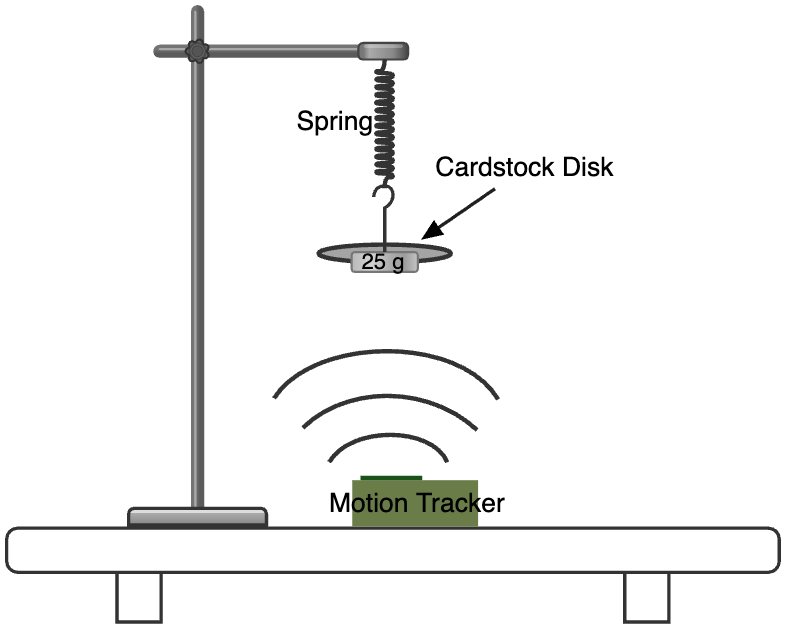
\includegraphics[width=4in]{images/setup.png}
     \caption{A diagram of our experimental setup}
     \label{fig:setup}
 \end{figure}

% \pagebreak
\section{Procedure}

 We used the compass and scissors to cut out four circles of 4 cm, 6 cm, 8 cm, and 10 cm. We hung the spring vertically on the horizontal retort clamp, and measured it's equilibrium position. Then we attached the weight hanger (5 g) and placed 40 g of weight on it. We then measured the new equilibrium position. Then we reduced the total weight on the spring to 25 g to capture more exaggerated data, placed the motion sensor beneath, and did 5 30-second motion recordings. The first one had only the 25 g, but the second had the 4cm disk, the third the 6 cm disk, the fourth the 8cm disk, and the fifth the 10 cm disk. On each run, we held the spring as far up as possible, so that the spring was at it's 0 g equilibrium position. We then began recording and released it.

\section{Results}

First, we attempted to get a measurement of the spring constant. To do this, we measured the displacement of the springs equilibrium at 45 ± 1 g to be $23.4$ cm $=0.234$ ± 0.001 m. Let's derive how to find $k$:

\begin{align*}
    \sum F&=ma = 0 \\
    F_S-F_G&=ma = 0 \\
    -k\Delta x+mg&=ma = 0 \\
    k\Delta x&=mg
\end{align*}
\begin{equation}
    k=\frac{mg}{\Delta x}
\end{equation}

Let us substitute in our numbers:

\begin{equation*}
    k=\frac{0.045 \pm 0.001 \text{ kg} \times 9.81 \frac{\text{m}}{\text{s}^2}}{0.234 \pm 0.001 \text{ m}} = \mathbf{1.90 \pm 0.04} \frac{\textbf{kg}}{\textbf{s}^\mathbf{2}}
\end{equation*}

After collecting data in Labquest, we exported the five runs as a single text file with time, position, velocity, and acceleration. Then I used a Python script that I wrote (see \url{https://github.com/benonymity/PHY-310/blob/main/Lab2/analysis.py}) to analyze and graph the data. First, it imports all data from the text file and then separates each run by rolling over when the time counter resets to zero. For each run, it averages all the data to normalize it around a center line so that I can center the data around the x-axis, which should be the equilibrium position. Then it finds the absolute value of each maximum and minimum, and fits those points to two curves; one described by the equation
\begin{equation}
    y=Ae^{-bt} + C
\label{eqn:envelope}
\end{equation}
Which is simply the envelope, or the damping term of the oscillation. It also fit the data to the ideal curve for the entire oscillation, represented by
\begin{equation}
    y=Ae^{-bt} \cos \left(\omega t + \phi\right) + C
\label{eqn:oscillation}
\end{equation}
This is derived from the analysis of the drag force, where $v$ is velocity and $D$ is the drag coefficient
\begin{equation}
    \label{eqn:drag}
    F_D=3\pi \mu Dv
\end{equation}
We use differential analysis to get the equation of motion for dampened harmonic oscillation, which in it's full form is
\begin{equation}
\label{eqn:final}
    y=Ae^{-\frac{b}{2m}t} \cos \left(\sqrt{\frac{k}{m} - \frac{b^2}{4m^2}} t + \phi\right)
\end{equation}
However, we can solve $\omega$ and $b$ (which is really something like $3\pi \mu D$) as simple constants. This fitting it not always as accurate, but shows the ideal, noiseless oscillation and how well the data conforms to it. Also note that I am equivocating slightly on $b$ here—Equations \ref{eqn:oscillation} and \ref{eqn:envelope} uses a plain $-b$, while Equation \ref{eqn:final} uses $-\frac{b}{2m}$ as the exponential. I will be fitting a simple constant coefficient of $t$ with my Python, but will later multiply this by $2m$ to make it a unitless quantity independent of changing mass.

After fitting the curves, we got five equations, whose constants are recorded in the two tables. Table \ref{tab:envelope} has all the constants for the curve fit to the envelope equation (Equation \ref{eqn:envelope}), while Table \ref{tab:oscillation} is for the curve fit to the entire oscillatory equation (Equation \ref{eqn:oscillation}).

\begin{table}[ht]
\centering
\begin{tabular}{llllll}
                                & Area                            & Mass                         & $A$                          & $b$                          & $C$                          \\ \cline{2-6} 
\multicolumn{1}{l|}{No Disk}    & \multicolumn{1}{l|}{13 cm$^2$}  & \multicolumn{1}{l|}{25.00 g} & \multicolumn{1}{l|}{0.10170} & \multicolumn{1}{l|}{0.01695} & \multicolumn{1}{l|}{0.03657} \\ \cline{2-6} 
\multicolumn{1}{l|}{4 cm Disk}  & \multicolumn{1}{l|}{50 cm$^2$}  & \multicolumn{1}{l|}{25.99g}  & \multicolumn{1}{l|}{0.10584} & \multicolumn{1}{l|}{0.06679} & \multicolumn{1}{l|}{0.01263} \\ \cline{2-6} 
\multicolumn{1}{l|}{6 cm Disk}  & \multicolumn{1}{l|}{113 cm$^2$} & \multicolumn{1}{l|}{27.43 g} & \multicolumn{1}{l|}{0.11132} & \multicolumn{1}{l|}{0.17353} & \multicolumn{1}{l|}{0.00989} \\ \cline{2-6} 
\multicolumn{1}{l|}{8 cm Disk}  & \multicolumn{1}{l|}{201 cm$^2$} & \multicolumn{1}{l|}{28.95 g} & \multicolumn{1}{l|}{0.12131} & \multicolumn{1}{l|}{0.27732} & \multicolumn{1}{l|}{0.00495} \\ \cline{2-6} 
\multicolumn{1}{l|}{10 cm Disk} & \multicolumn{1}{l|}{314 cm$^2$} & \multicolumn{1}{l|}{31.32 g} & \multicolumn{1}{l|}{0.15710} & \multicolumn{1}{l|}{0.45115} & \multicolumn{1}{l|}{0.00571} \\ \cline{2-6} 
\end{tabular}
\caption{Constants in Envelope Fit}
\label{tab:envelope}
\end{table}

\begin{table}[ht]
\centering
\begin{tabular}{llllllll}
                                & Area                            & Mass                         & $A$                          & $b$                          & $C$                          & $\omega$                     & $\phi$                        \\ \cline{2-8} 
\multicolumn{1}{l|}{No Disk}    & \multicolumn{1}{l|}{13 cm$^2$}  & \multicolumn{1}{l|}{25.00 g} & \multicolumn{1}{l|}{0.10168} & \multicolumn{1}{l|}{0.01699} & \multicolumn{1}{l|}{0.00017} & \multicolumn{1}{l|}{7.84299} & \multicolumn{1}{l|}{0.65649}  \\ \cline{2-8} 
\multicolumn{1}{l|}{4 cm Disk}  & \multicolumn{1}{l|}{50 cm$^2$}  & \multicolumn{1}{l|}{25.99g}  & \multicolumn{1}{l|}{0.11307} & \multicolumn{1}{l|}{0.05288} & \multicolumn{1}{l|}{0.00016} & \multicolumn{1}{l|}{7.66648} & \multicolumn{1}{l|}{–1.81840} \\ \cline{2-8} 
\multicolumn{1}{l|}{6 cm Disk}  & \multicolumn{1}{l|}{113 cm$^2$} & \multicolumn{1}{l|}{27.43 g} & \multicolumn{1}{l|}{0.11154} & \multicolumn{1}{l|}{0.12032} & \multicolumn{1}{l|}{0.00049} & \multicolumn{1}{l|}{7.39021} & \multicolumn{1}{l|}{–2.23723} \\ \cline{2-8} 
\multicolumn{1}{l|}{8 cm Disk}  & \multicolumn{1}{l|}{201 cm$^2$} & \multicolumn{1}{l|}{28.95 g} & \multicolumn{1}{l|}{0.12103} & \multicolumn{1}{l|}{0.19301} & \multicolumn{1}{l|}{0.00030} & \multicolumn{1}{l|}{7.12469} & \multicolumn{1}{l|}{–1.85440} \\ \cline{2-8} 
\multicolumn{1}{l|}{10 cm Disk} & \multicolumn{1}{l|}{314 cm$^2$} & \multicolumn{1}{l|}{31.32 g} & \multicolumn{1}{l|}{0.14428} & \multicolumn{1}{l|}{0.31610} & \multicolumn{1}{l|}{0.00050} & \multicolumn{1}{l|}{6.69661} & \multicolumn{1}{l|}{–2.01379} \\ \cline{2-8} 
\end{tabular}
\caption{Constants in Oscillation Fit}
\label{tab:oscillation}
\end{table}

Analyzing these constants to find a relationship between damping constant and cross-sectional area requires us to make b independent of mass, as each time we change out the card-stock disk, there is a subtle change in mass on the spring. To do this, we'll multiply each of our fitted "$b$" (which actually represents $\frac{b}{2m}$ in Equation \ref{eqn:final}) values by $2m$ to remove that changing variable and isolate $b$ as it changes with area. See Table \ref{tab:barea}.

\begin{figure}[H]
\centering
\minipage{0.5\textwidth}
  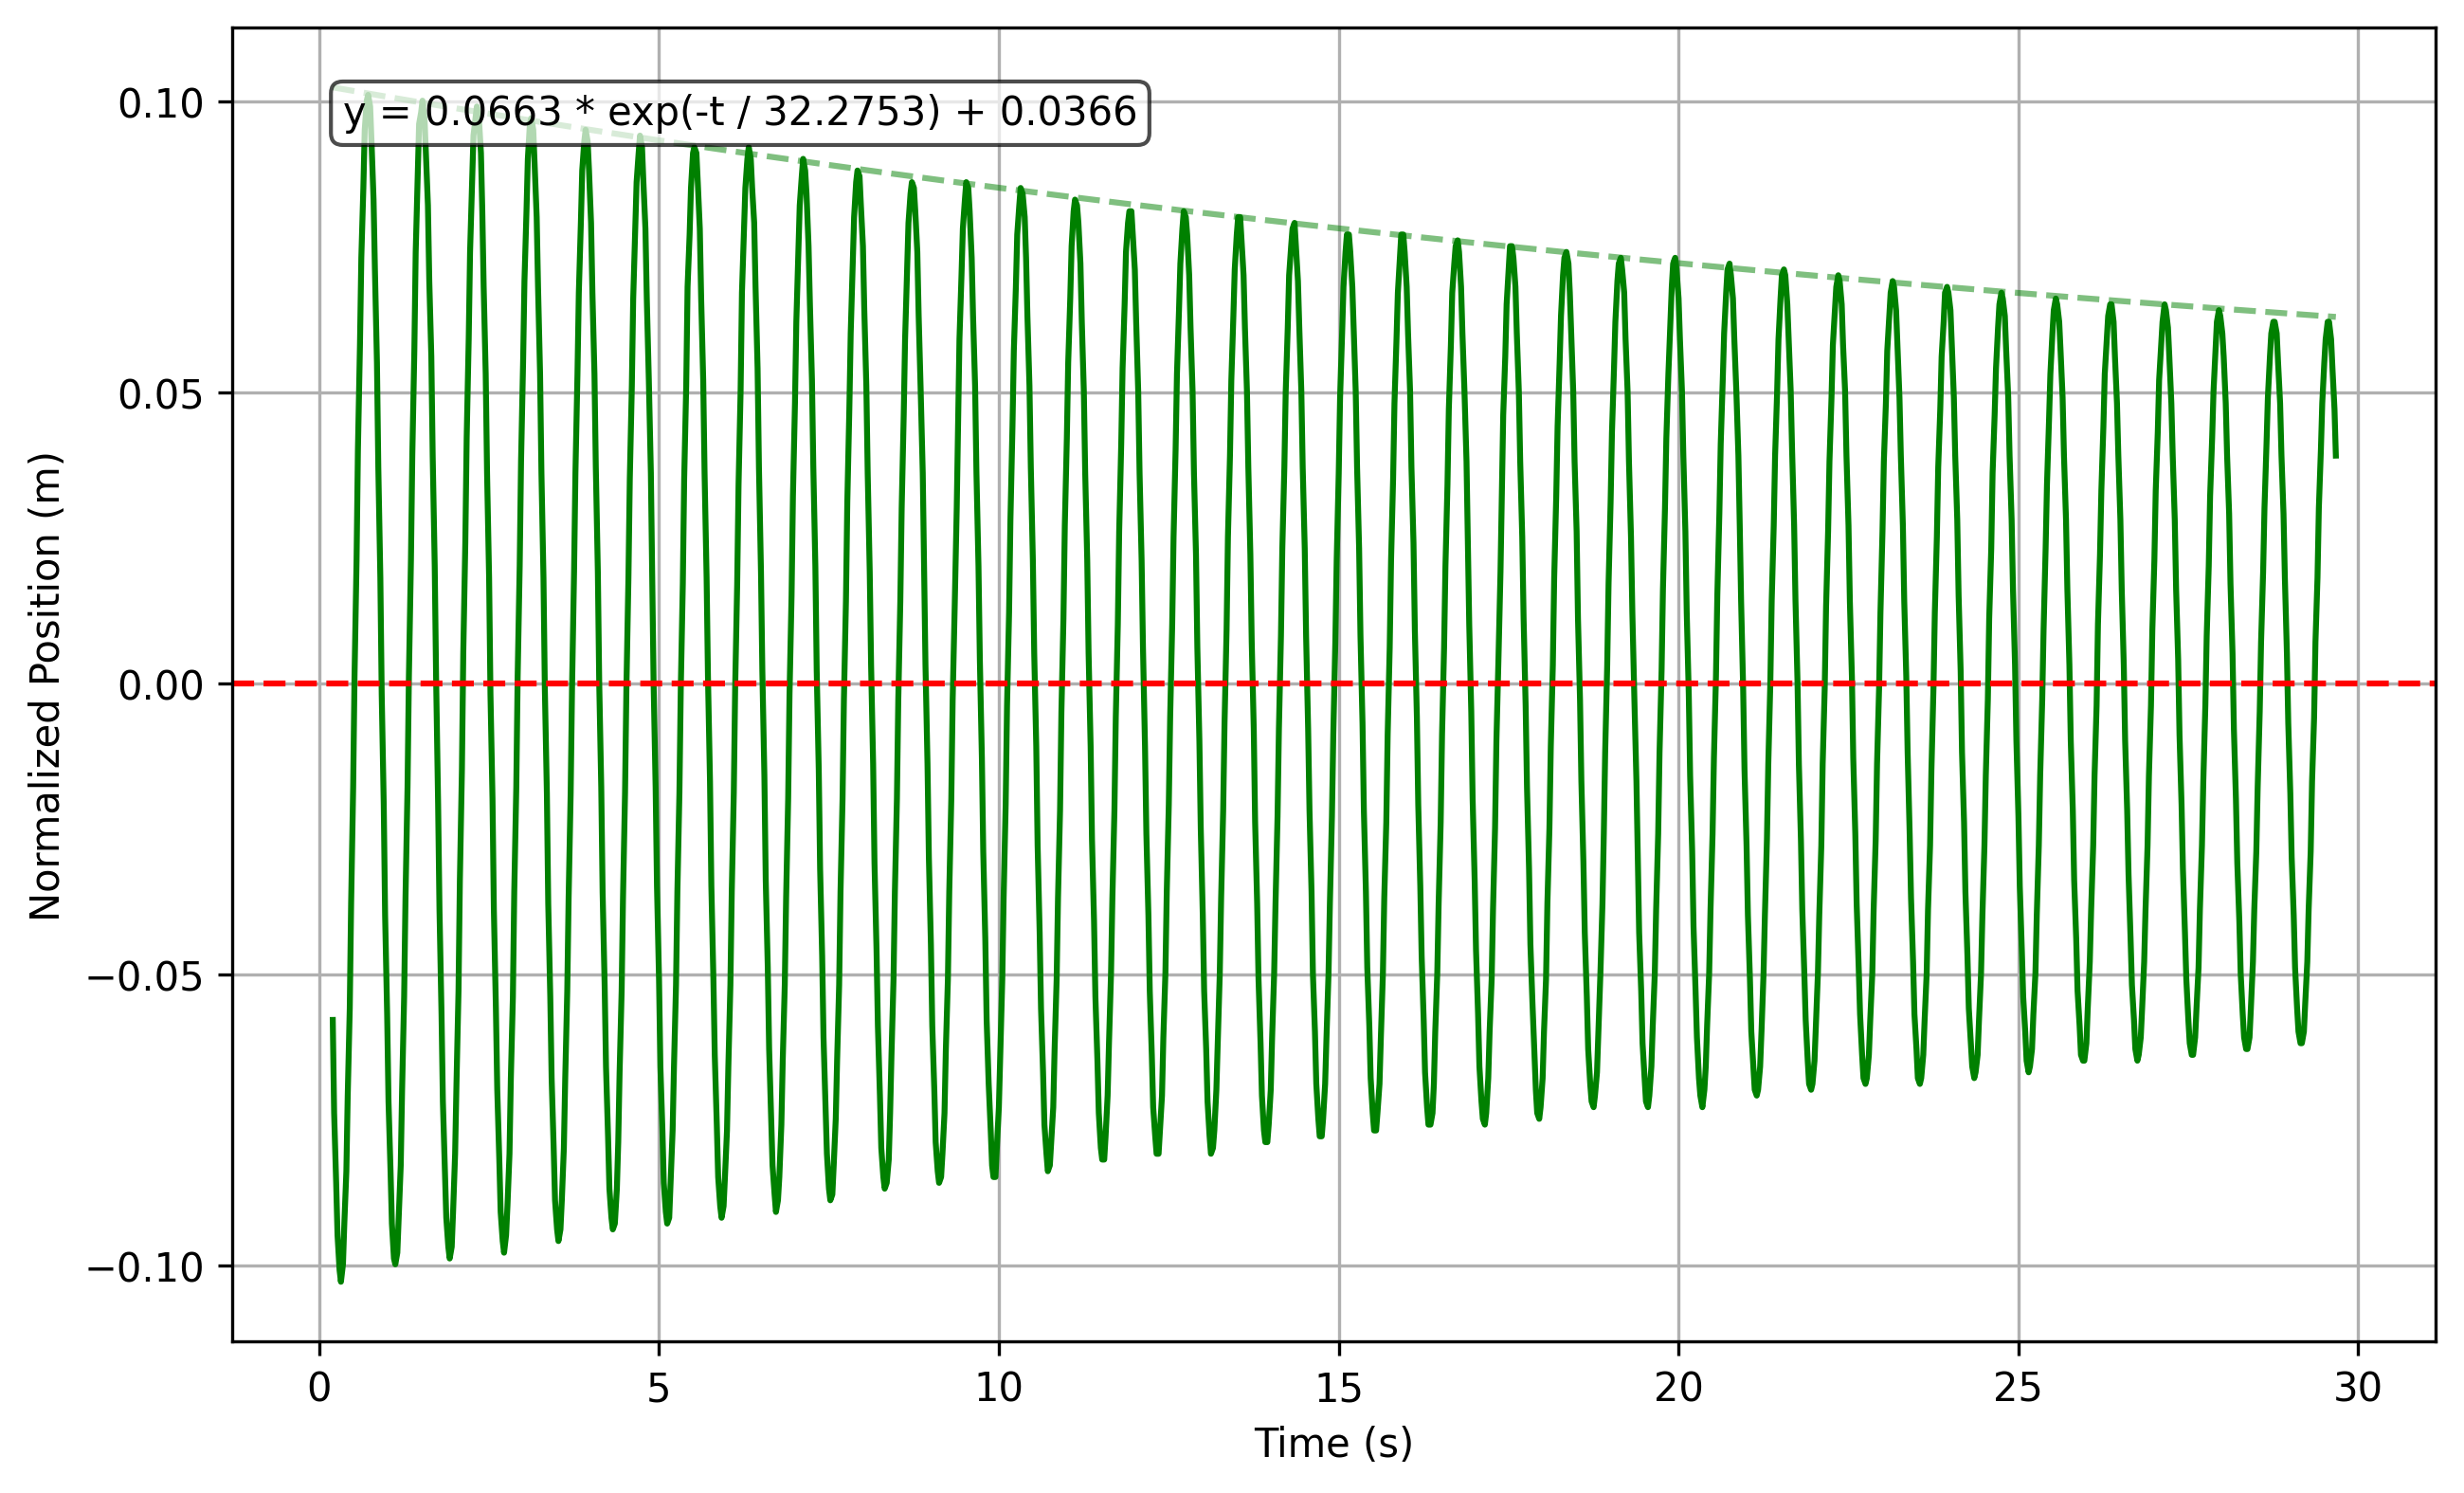
\includegraphics[width=\linewidth]{images/2cm.png}
  \caption{Spring with only 25g}\label{fig:2cm}
\endminipage\hfill
\minipage{0.5\textwidth}
  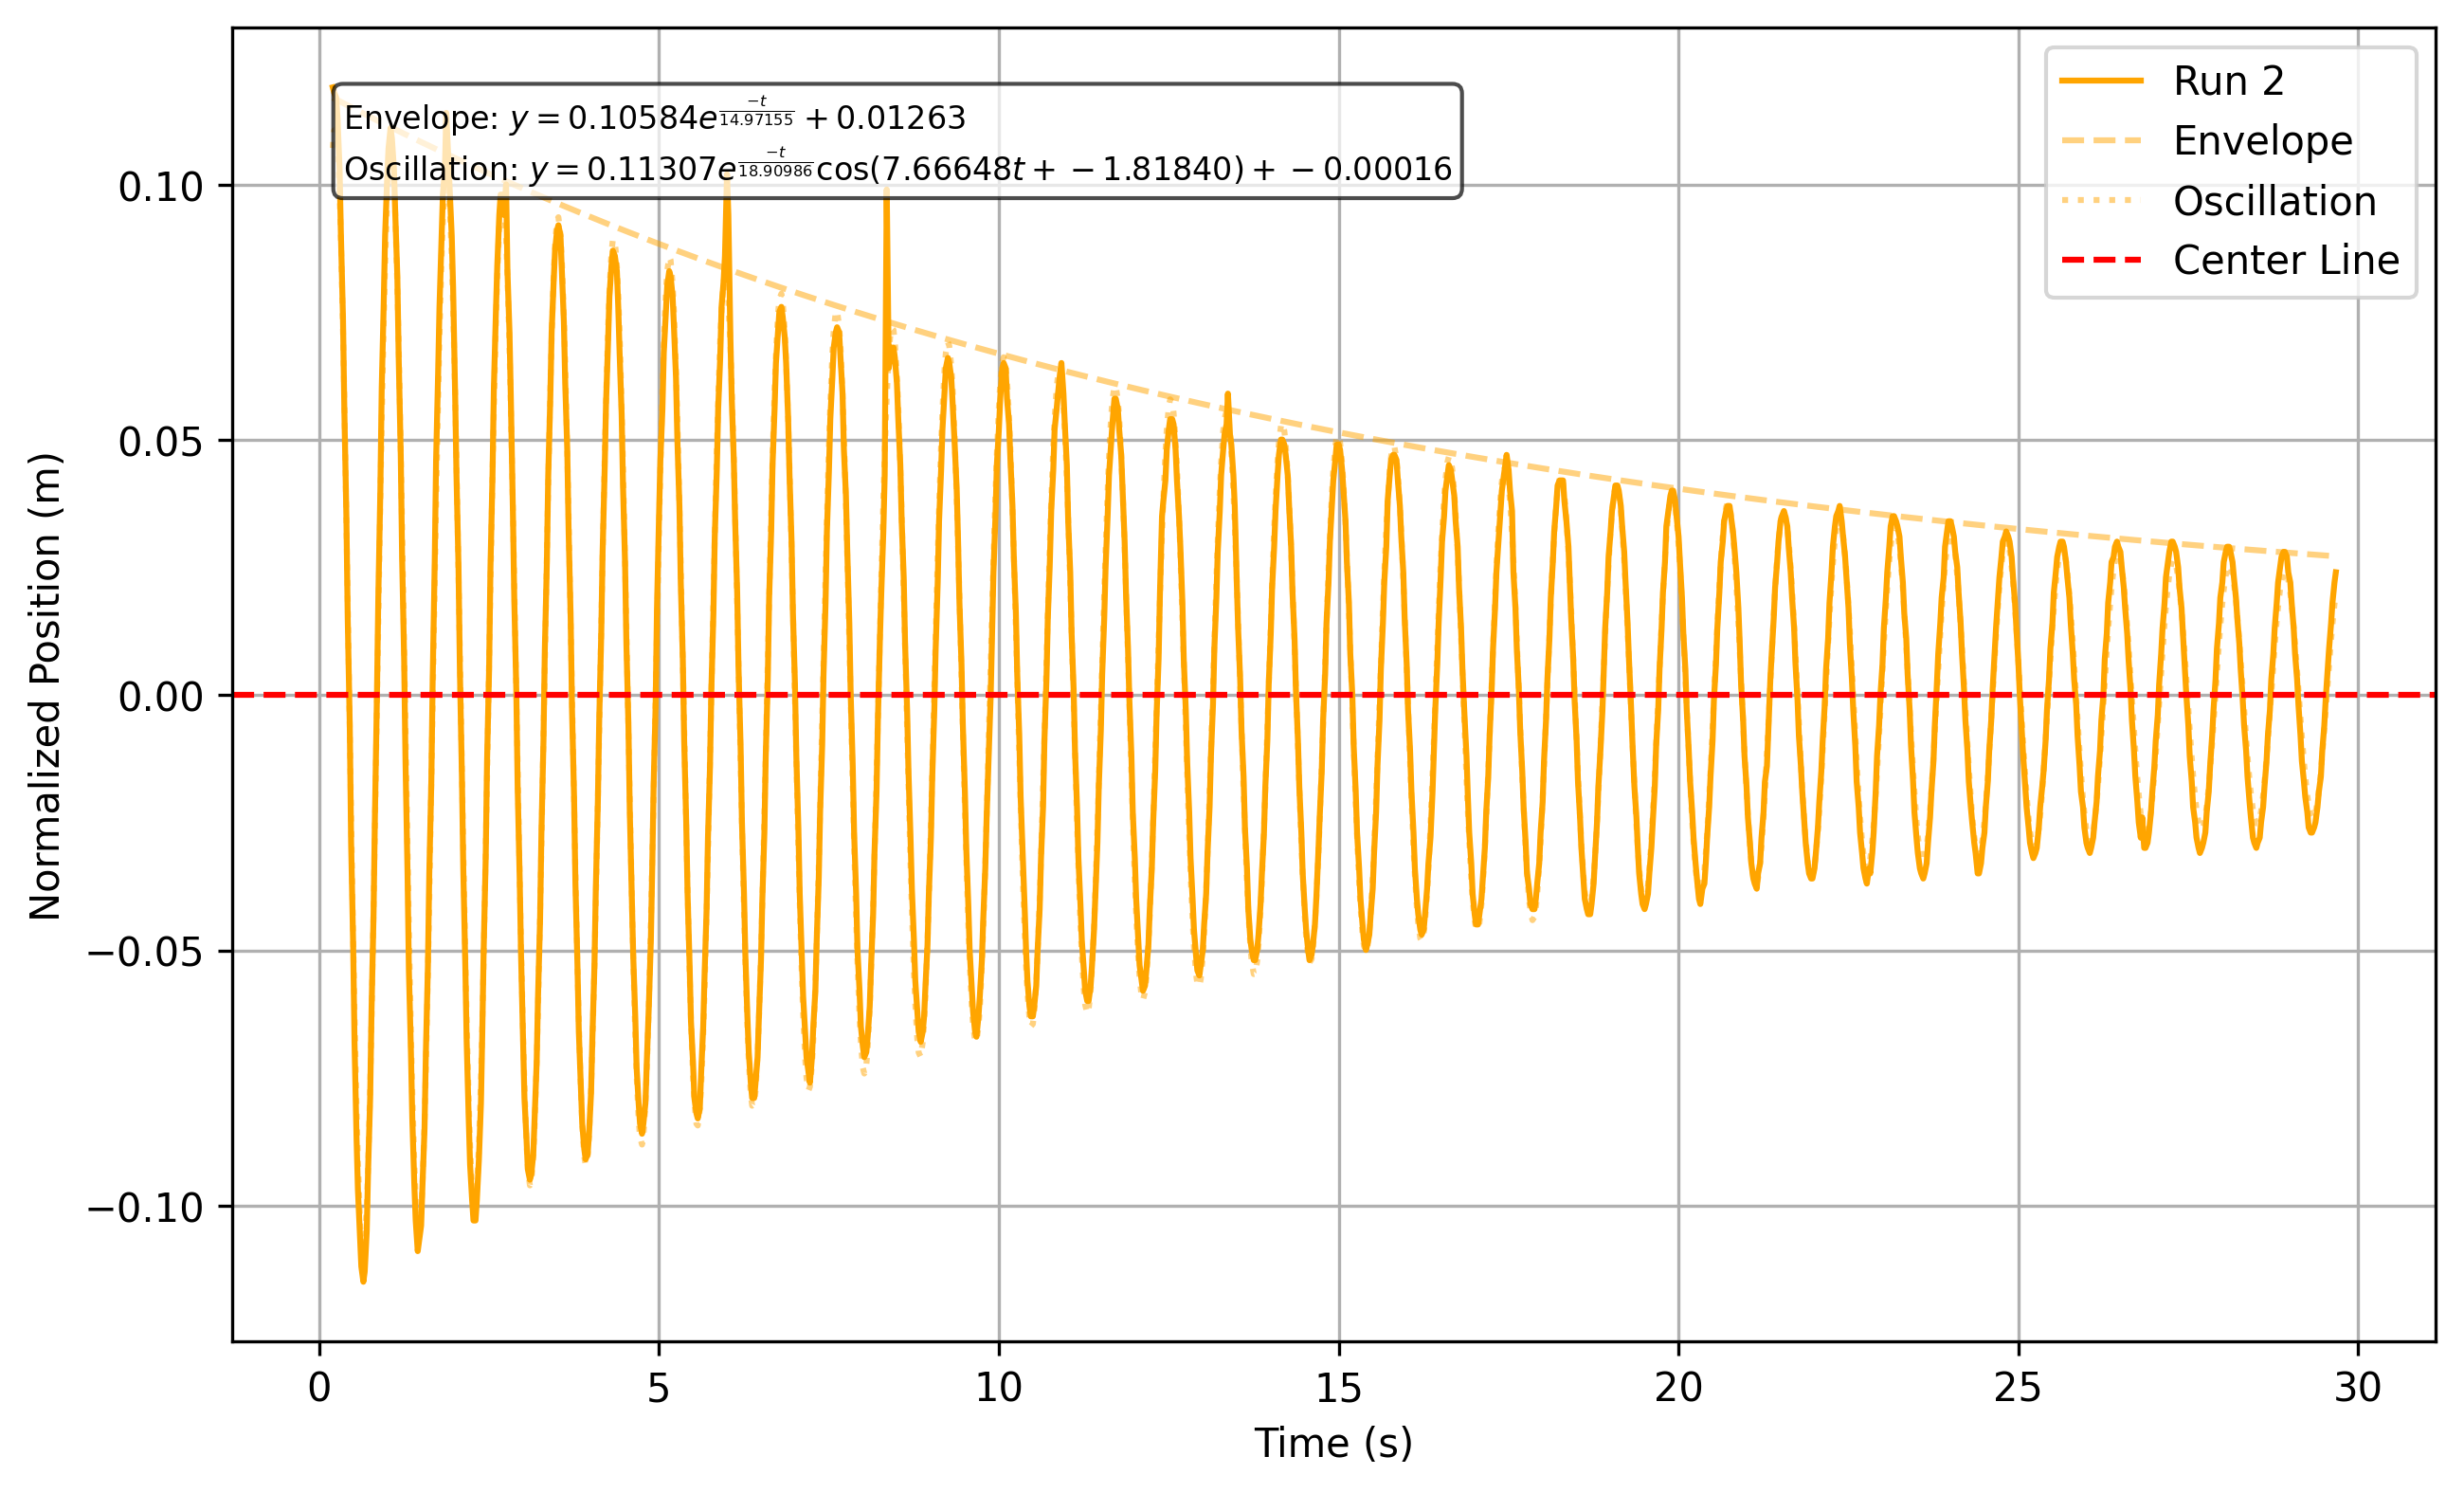
\includegraphics[width=\linewidth]{images/4cm.png}
  \caption{Spring with 25g and a 4cm disk}\label{fig:4cm}
\endminipage\hfill
\\
\minipage{0.5\textwidth}
  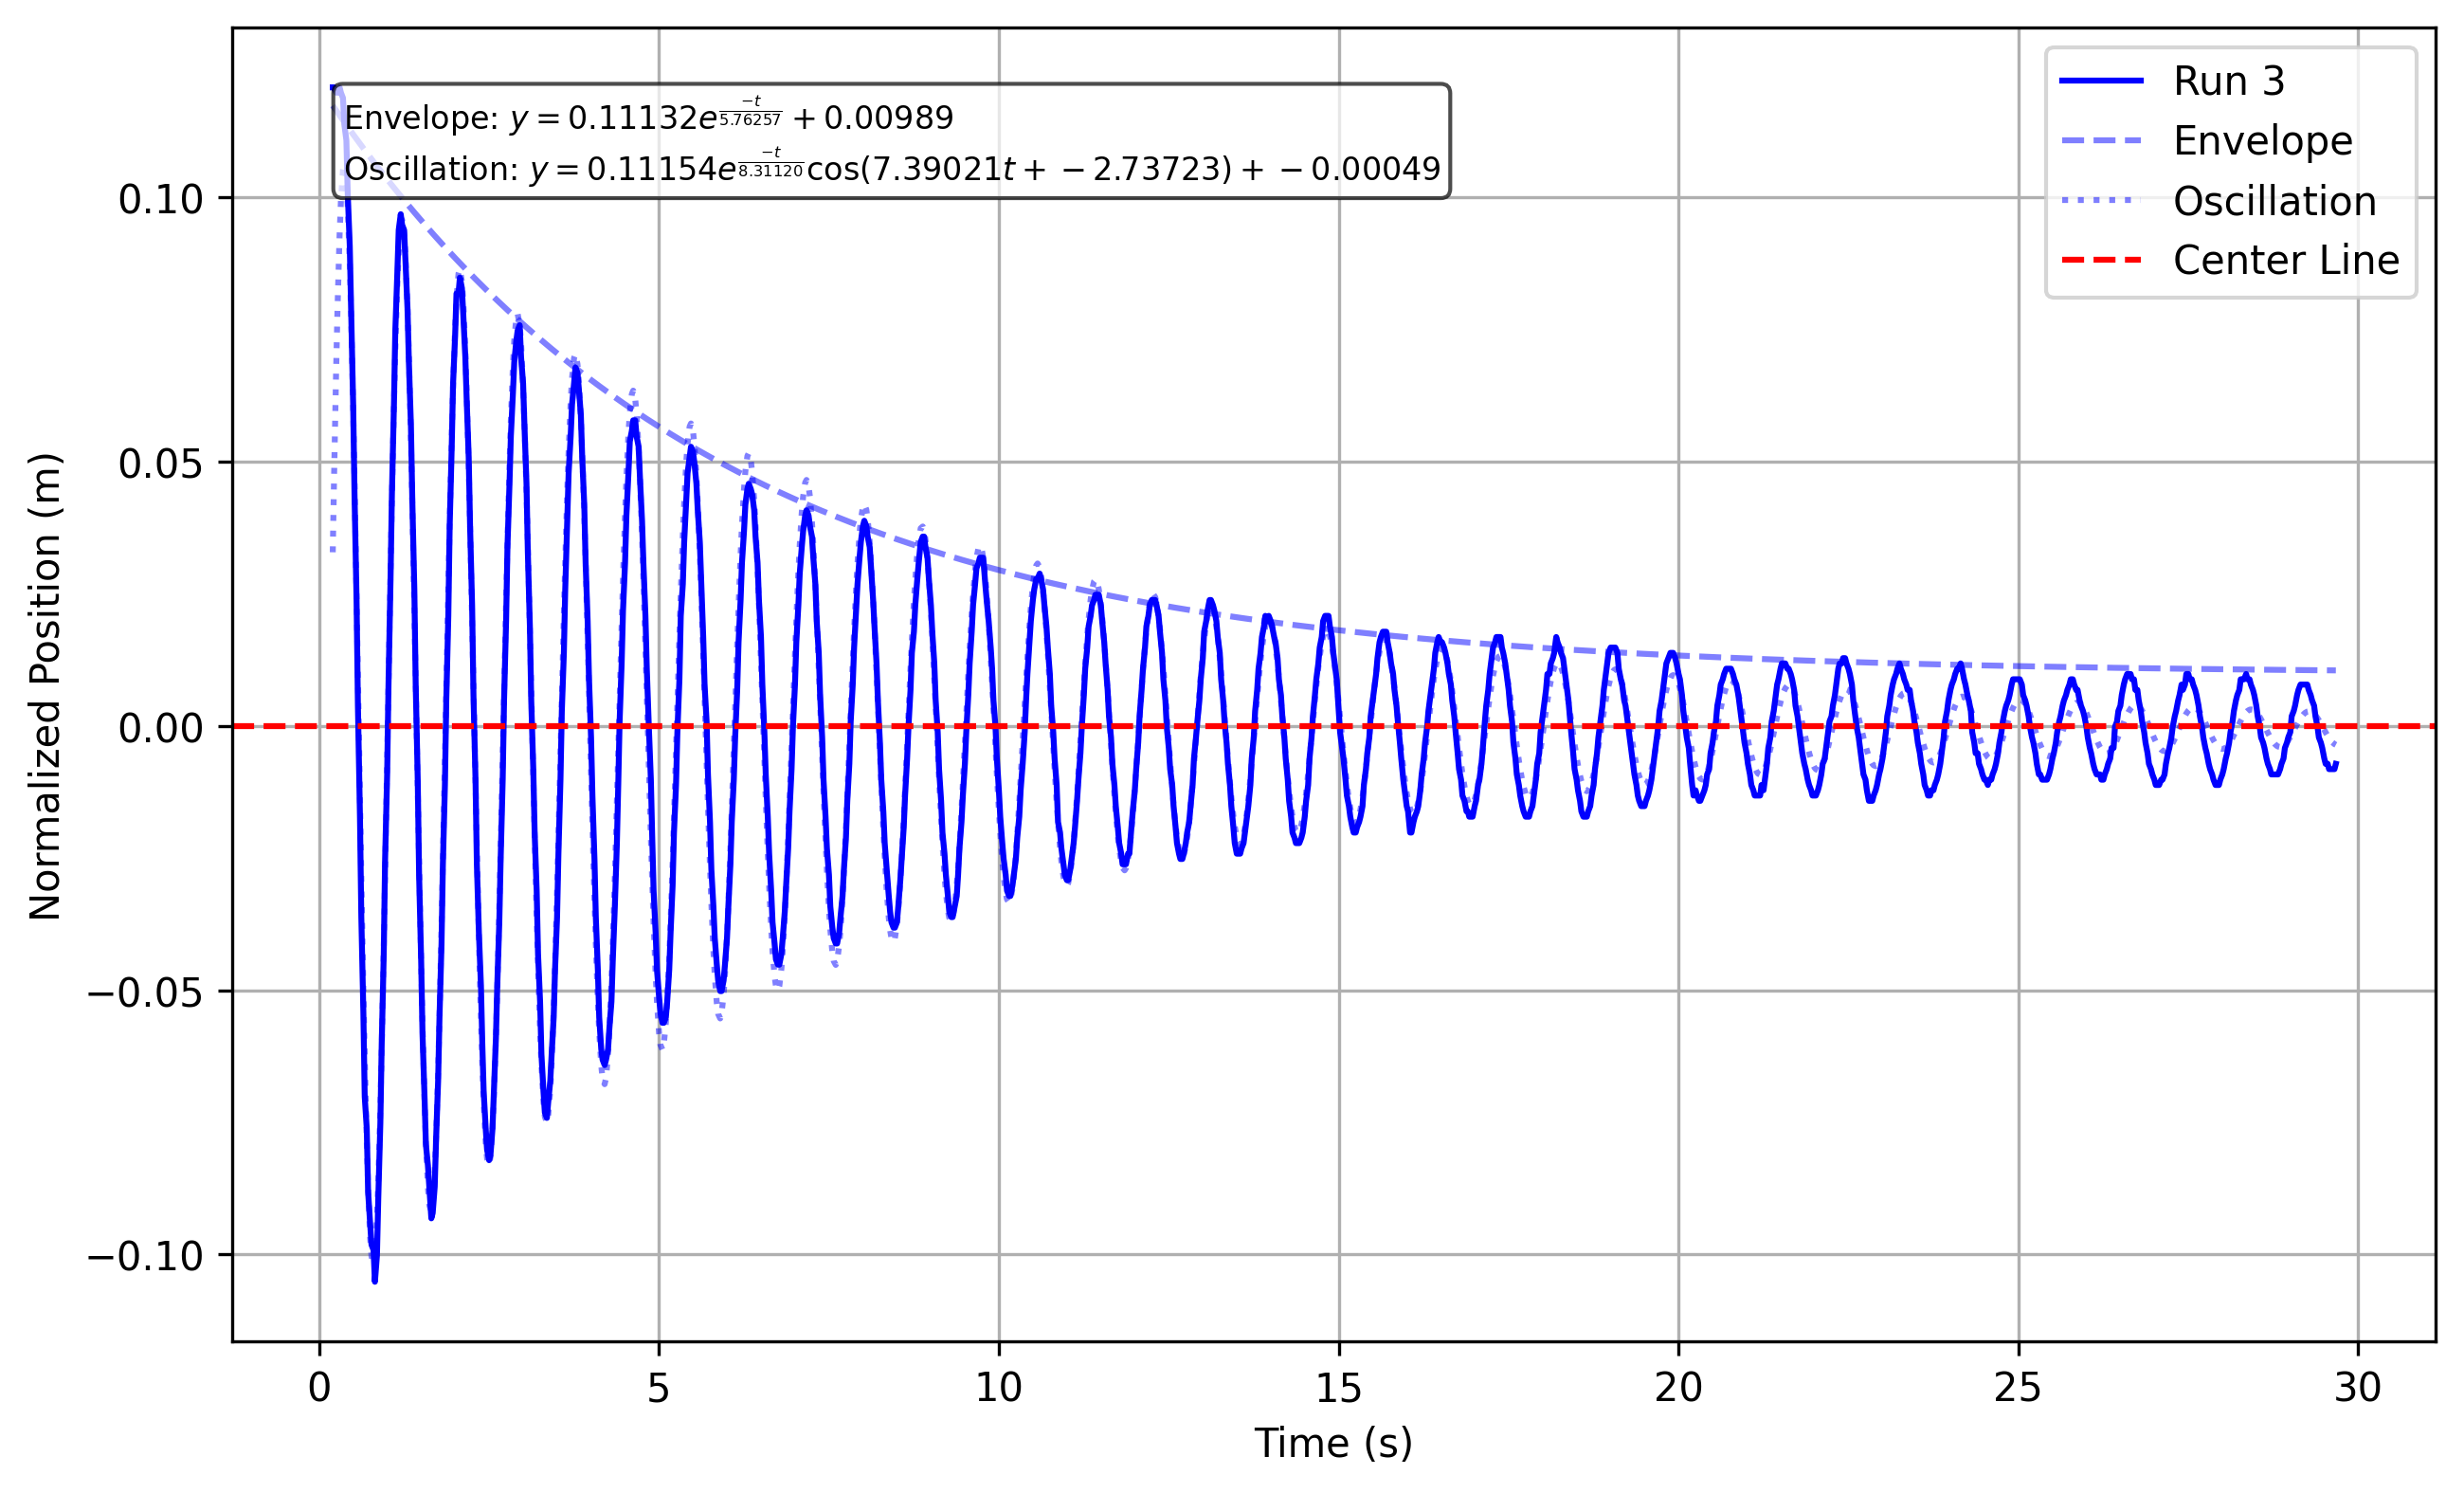
\includegraphics[width=\linewidth]{images/6cm.png}
  \caption{Spring with 25g and a 6cm disk}\label{fig:6cm}
\endminipage\hfill
\minipage{0.5\textwidth}
  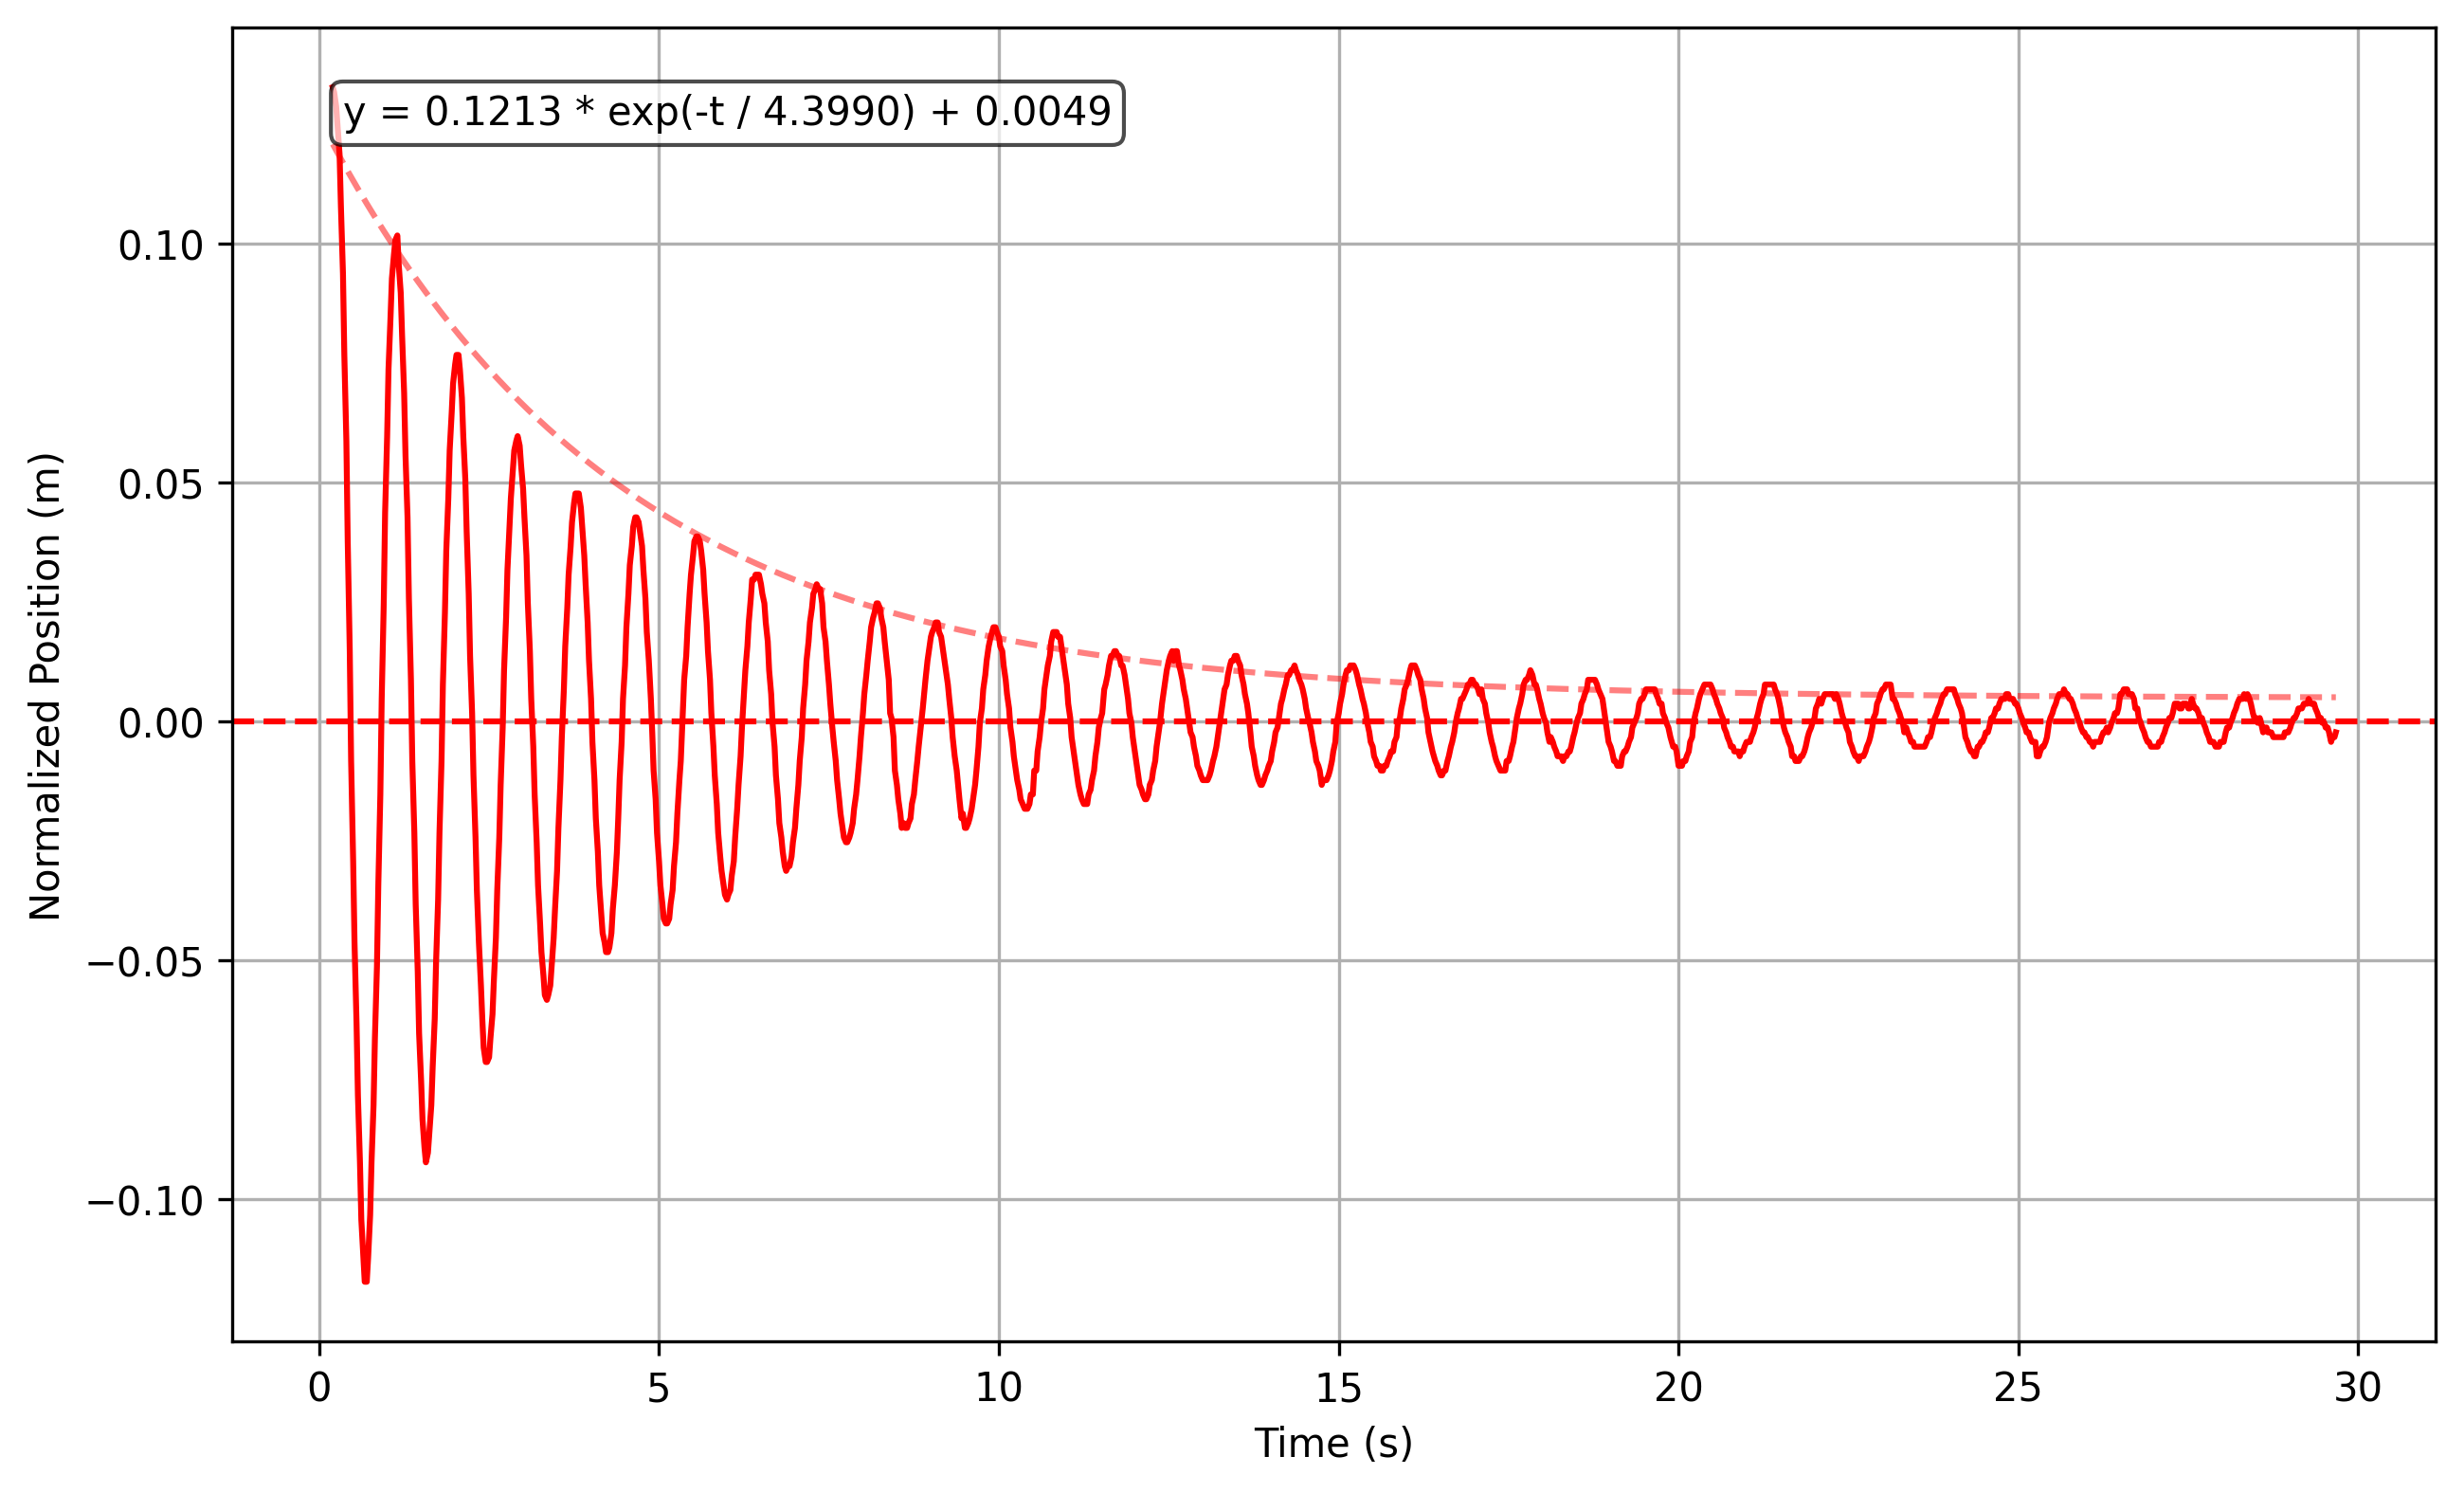
\includegraphics[width=\linewidth]{images/8cm.png}
  \caption{Spring with 25g and a 8cm disk}\label{fig:8cm}
\endminipage\hfill
\\
\minipage{0.5\textwidth}
% \begin{figure}[ht]
  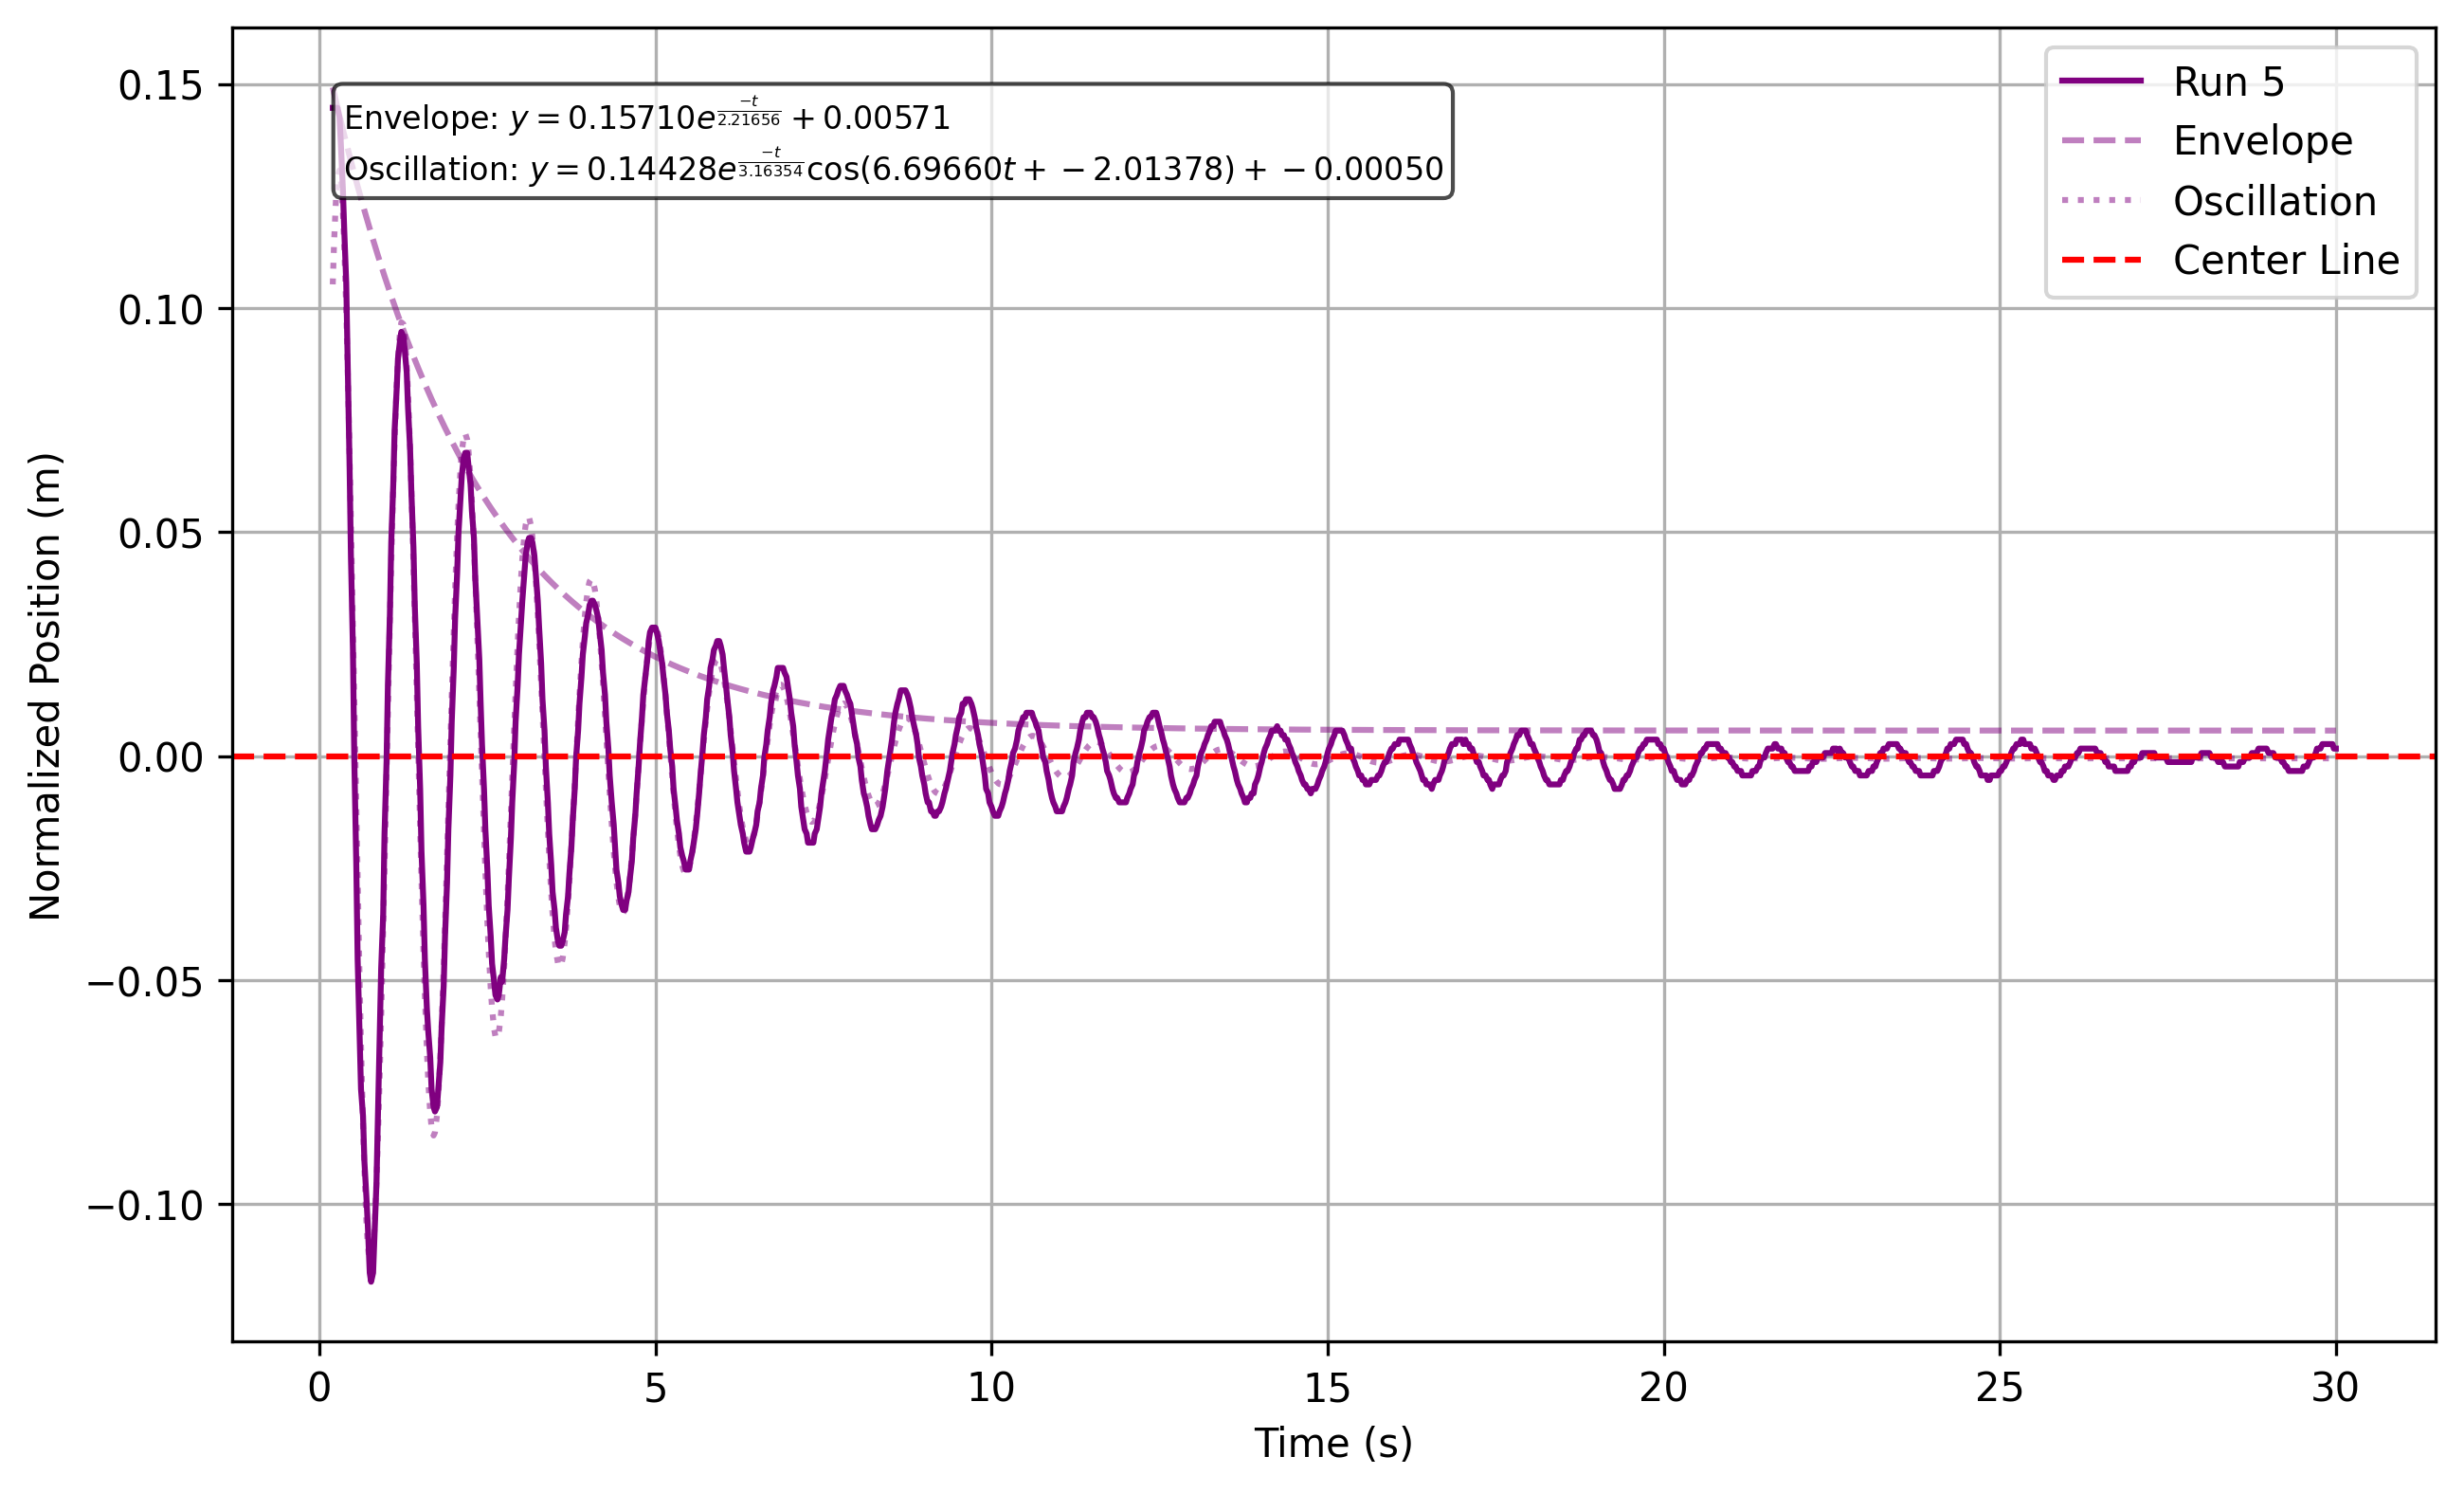
\includegraphics[width=\linewidth]{images/10cm.png}
  \caption{Spring with 25g and a 10cm disk}\label{fig:10cm}
% \end{figure}
\endminipage
\end{figure}

\begin{table}[ht]
\centering
\begin{tabular}{lllll}
                                & Area                            & Mass                         & Oscillation $b\times 2m$ & Envelope $b\times 2m$ \\ \cline{2-5} 
\multicolumn{1}{l|}{No Disk}    & \multicolumn{1}{l|}{13 cm$^2$}  & \multicolumn{1}{l|}{25.00 g} & \multicolumn{1}{l|}{0.4248}             & \multicolumn{1}{l|}{0.4238}          \\ \cline{2-5} 
\multicolumn{1}{l|}{4 cm Disk}  & \multicolumn{1}{l|}{50 cm$^2$}  & \multicolumn{1}{l|}{25.99g}  & \multicolumn{1}{l|}{1.374}              & \multicolumn{1}{l|}{1.736}           \\ \cline{2-5} 
\multicolumn{1}{l|}{6 cm Disk}  & \multicolumn{1}{l|}{113 cm$^2$} & \multicolumn{1}{l|}{27.43 g} & \multicolumn{1}{l|}{3.300}              & \multicolumn{1}{l|}{4.760}           \\ \cline{2-5} 
\multicolumn{1}{l|}{8 cm Disk}  & \multicolumn{1}{l|}{201 cm$^2$} & \multicolumn{1}{l|}{28.95 g} & \multicolumn{1}{l|}{5.588}              & \multicolumn{1}{l|}{8.028}           \\ \cline{2-5} 
\multicolumn{1}{l|}{10 cm Disk} & \multicolumn{1}{l|}{314 cm$^2$} & \multicolumn{1}{l|}{31.32 g} & \multicolumn{1}{l|}{9.900}              & \multicolumn{1}{l|}{14.13}           \\ \cline{2-5} 
\end{tabular}
\caption{Adjusted $b$ Values w.r.t. Area}
\label{tab:barea}
\end{table}

After isolating $b$ with respect to area, we graph it as shown in Figure \ref{fig:benv} and Figure \ref{fig:bosc}, which shows us that there is a linear relationship of $b$ and area. Increase the cross-sectional area, and $b$ will increase linearly with it, prefixed by some constant slope ($\approx3\pi\mu$).

\begin{figure}[ht]
    \centering
    \minipage{0.7\textwidth}
      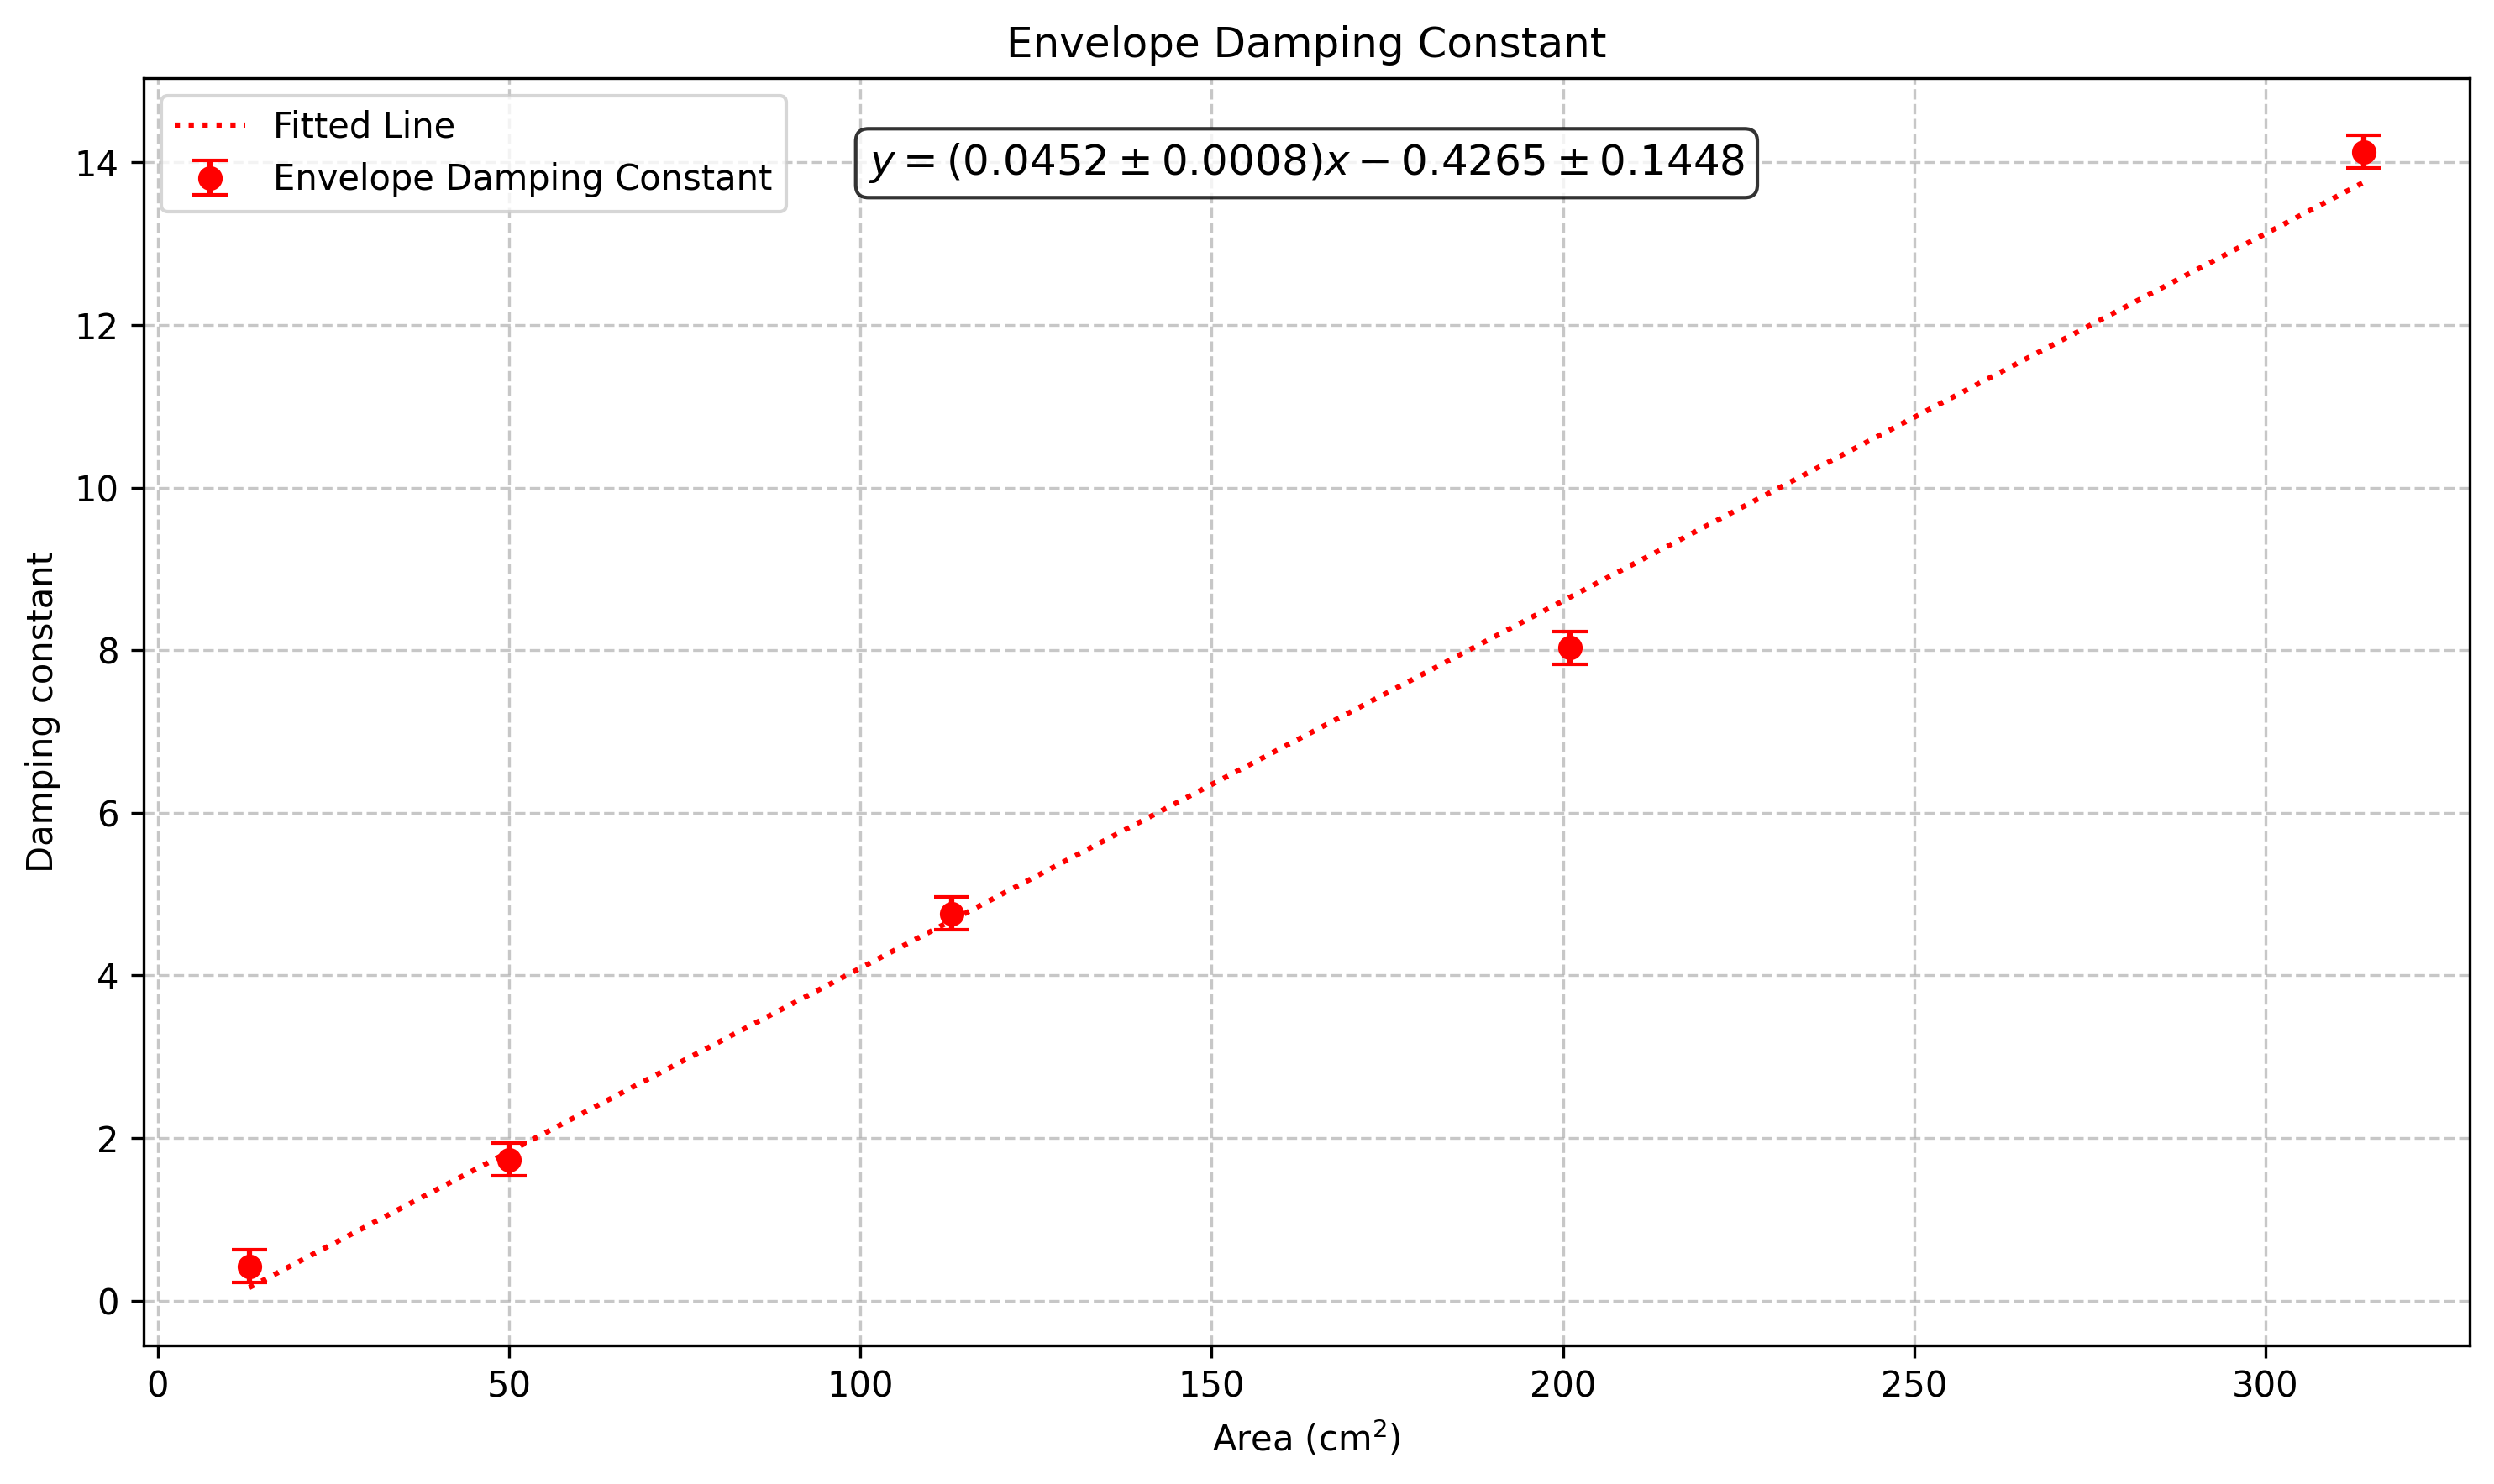
\includegraphics[width=\linewidth]{images/b-area_envelope_damping_constant.png}
      \caption{$b$ (from envelope) w.r.t. area}\label{fig:benv}
    \endminipage\hfill
    \minipage{0.7\textwidth}
      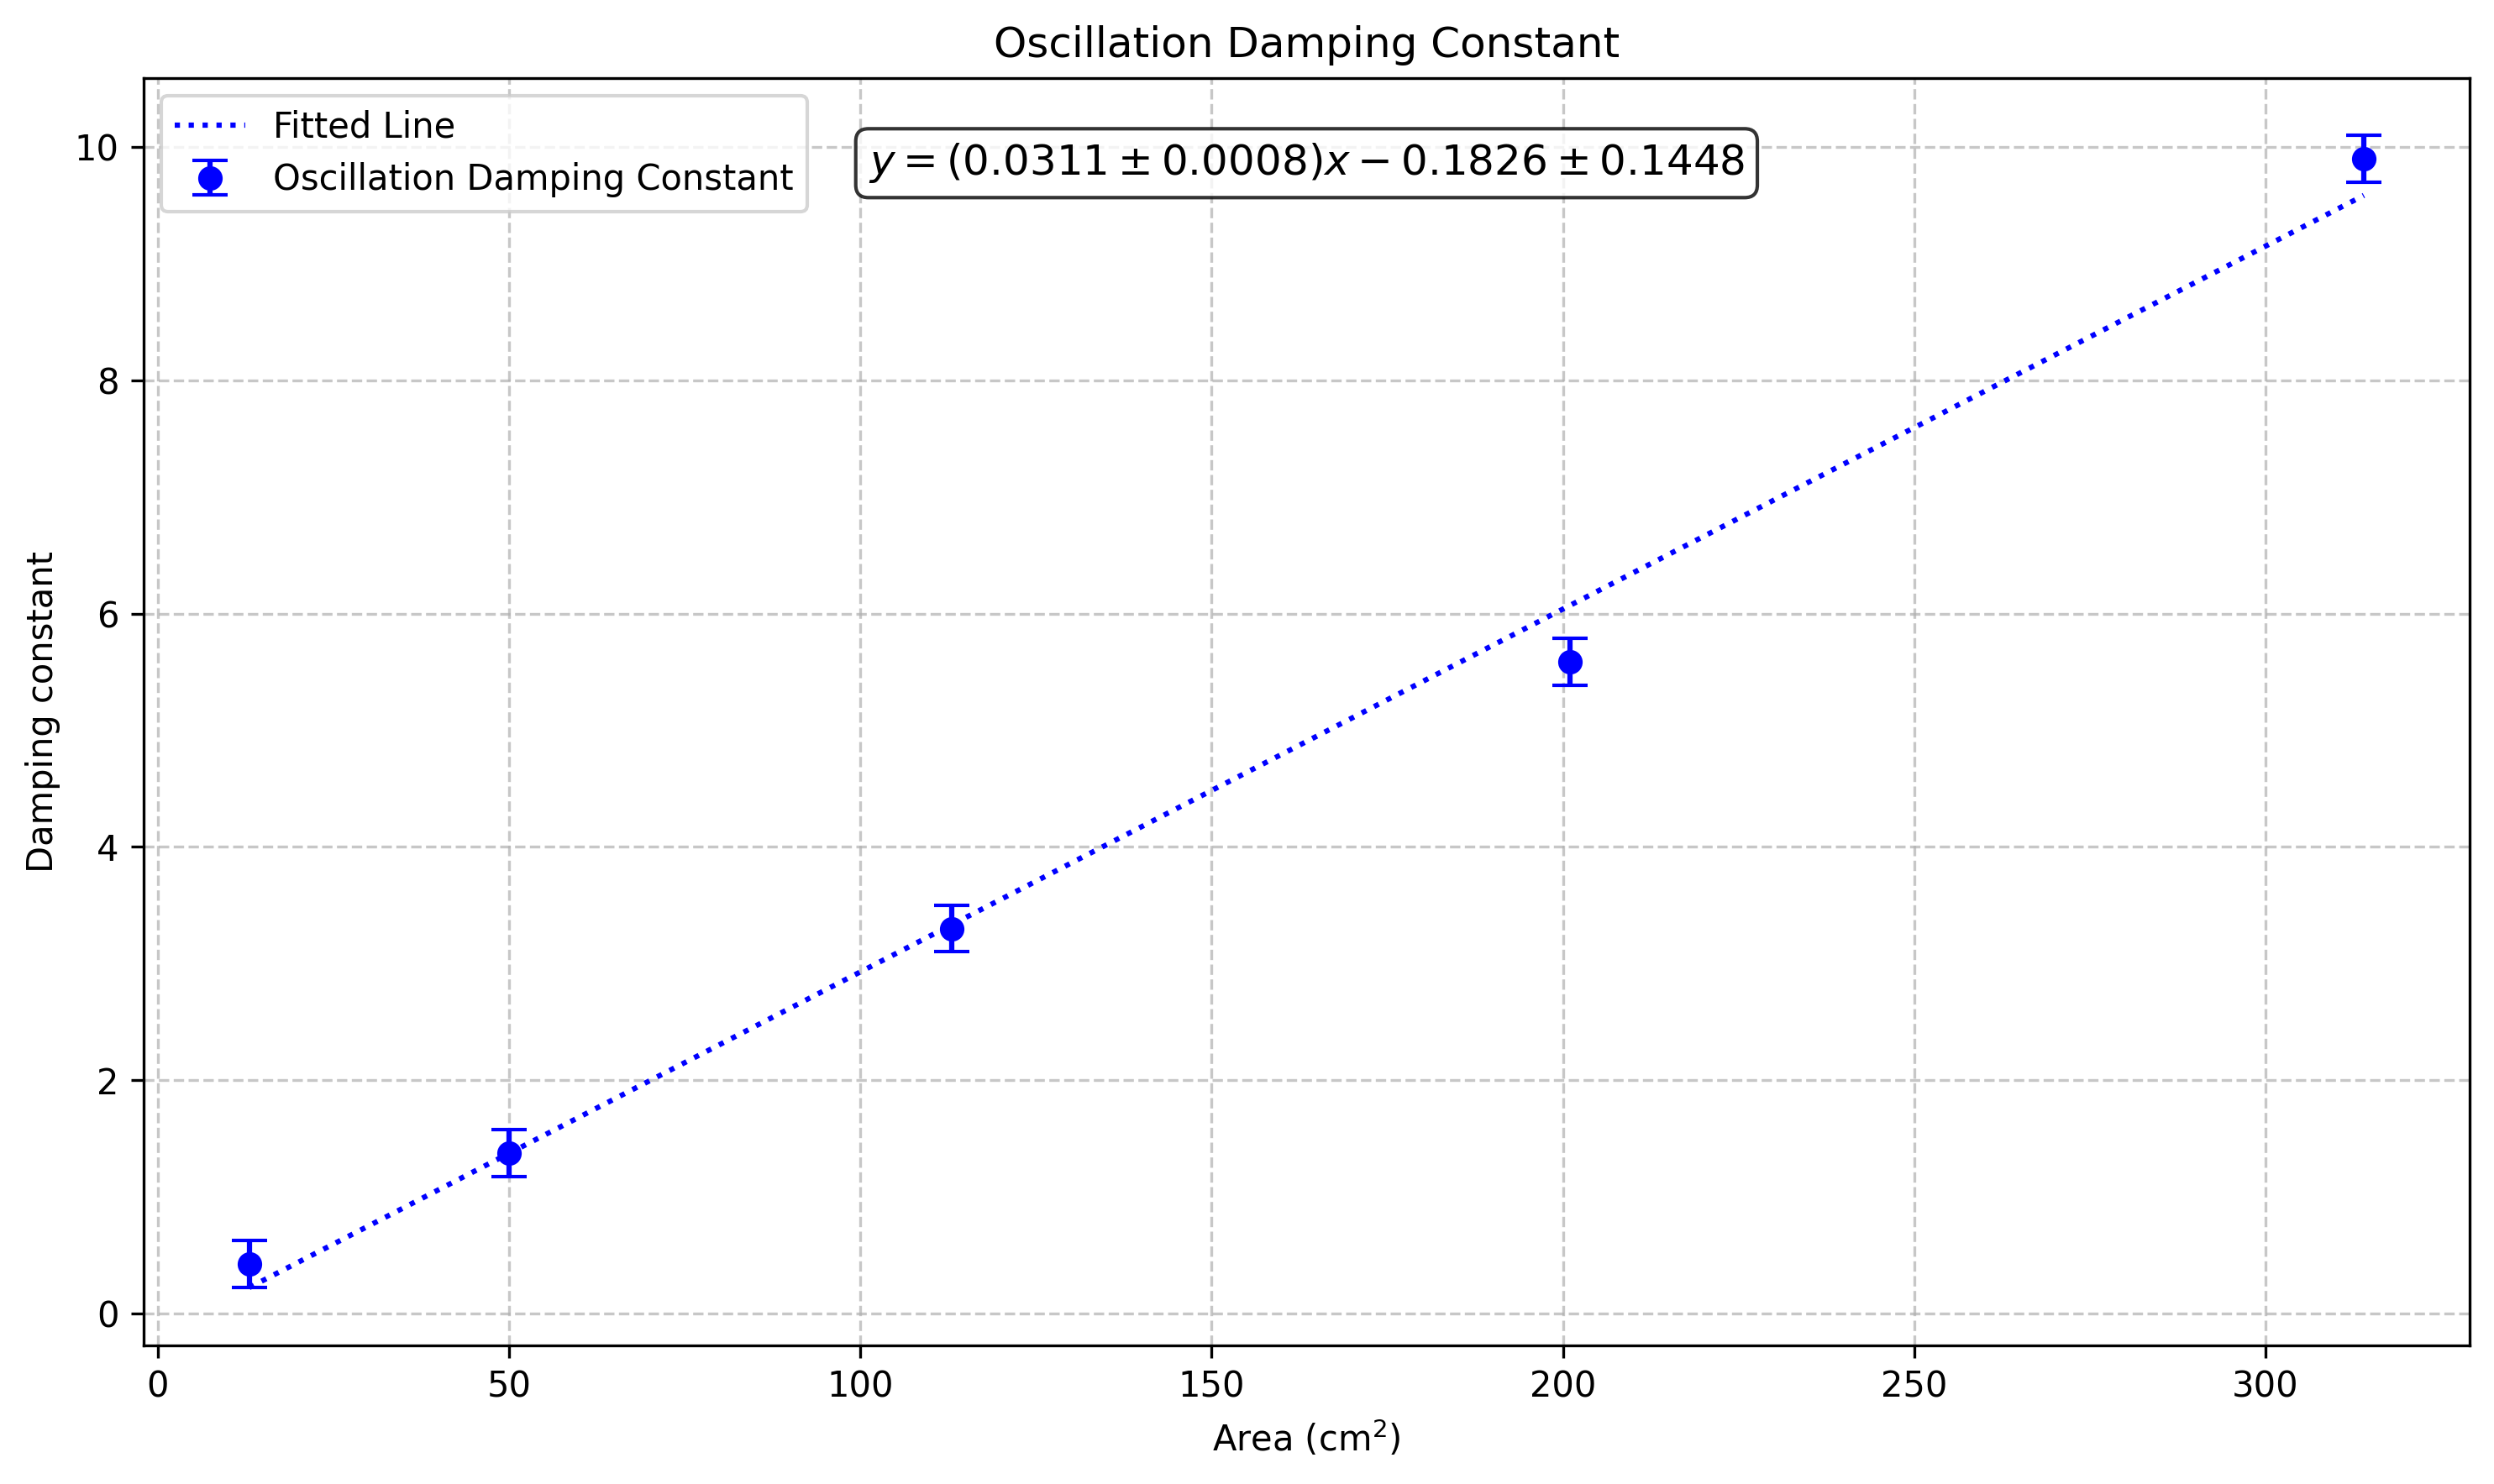
\includegraphics[width=\linewidth]{images/b-area_oscillation_damping_constant.png}
      \caption{$b$ (from oscillation) w.r.t. area}\label{fig:bosc}
    \endminipage\hfill
\end{figure}

\section{Error}

All of the values in the tables are precise to more decimal points than our data was in (mm), but this is so we can carry those computed values through and round to significant digits at the end. All of the mass measurements were done on a scale that is $± 0.01$ g, and all of the motion sensor measurements were $± 1$ mm. We didn't do much actual math to these original values, but our error propagation still needs to be done. The b-values are computed by fit, so I simply carried the error from the position and mass data using the error propagation formula.

\begin{equation}
    \delta f=\sum_i \left(\frac{\delta f}{\delta a_i}\right)\delta a_i^2
\end{equation}

Incorporating error into the tables caused them to run off the page and seems unnecessary, so I simply added error bars into Figures \ref{fig:benv} and \ref{fig:bosc}.

Finally, the difference between the envelope and oscillation fits is often significant, raising some questions. However, this is likely due to the inconsistency in peaks vs. the consistency of the entirety of the curve. For instance, Figure \ref{fig:4cm} has two strange spikes on its peaks, and since the peaks are far more heavily weighted in the envelope equation vs. the oscillation one, such anomalies are less weighted. Our experimental setup was also imperfect, as we have no guarantee that some of the energy of the spring was going into horizontal shifts, as we could not lock the spring in into the vertical direction. The performing of this experiment in a lab with uncontrolled air currents also resulted in minute changes when the oscillations became extremely small, such as when a disk 10 cm in radius was oscillating in millimeters. It is hard to expect stable movement in such an unpredictable environment.

\section{Conclusions}

We observed a linear relationship between our circular cutouts (chosen so that their area could be easily measured, and to ensure uniform air flow, where something with sharp corners seems like it would introduce more turbulent flow.) This fits with our knowledge of Stokes' Law (Equation \ref{eqn:drag}), and shows us that increasing our surface area linearly increases our drag.

% \bibliographystyle{unsrtnat}
% \bibliography{references}

\end{document}
